\chapter{Methods and Experiments} \label{methods-and-experiments}

\section{Single-Agent Bilateral Negotiation Environment (\gls{sbe})}
In this environment, agent represents the negotiator in negotiation mechanism.

\subsection{Independent Negotiator in NegMAS}
In the environment has just single learnable \gls{drl} negotiator. All RL algorithms with the correct type of action space and observation space can be tested in this specific environment. In the experiment of this thesis, some algorithms, such as DQN, PPO, A2C, from stable-baselines \ref{backgrounds:stable-baselines} were tested in four learning cases:
\begin{itemize}
	\item single issue, acceptance strategy
	\item single issue, offer strategy
	\item multi-issues, acceptance strategy
	\item multi-issues, offer startegy
\end{itemize}

The training logic of some RL algorithms is shown in the figure \ref{fig:dqn}, and the detailed description of the algorithm is shown in the appendix \ref{appendix:dqn}.

\begin{figure}[htbp]
\centering
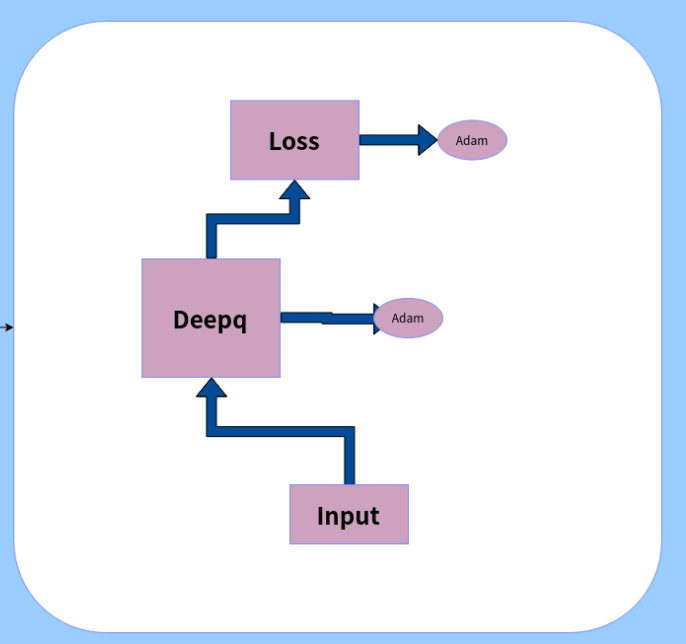
\includegraphics[width=0.30\textwidth]{./images/dqn.png}
\caption{Training logic of DQN}
\label{fig:dqn}
\end{figure}

\subsection{Experiment} \label{sbe:experiment}

Figure \ref{fig:bilateral-negotiation} diagrams the Game which consistes of two negotiators: RL negotiator and Opponent negotiator(AspirationNegotiator). Opponent Negotiator can be set in the configuration. All negotiators, which inherit the base abstract negotiator class in \gls{negmas} can be configured in the experiment. AspirationNegotiator is selected as the baseline negoitator in this experiment.

\begin{figure}[htbp]
\centering
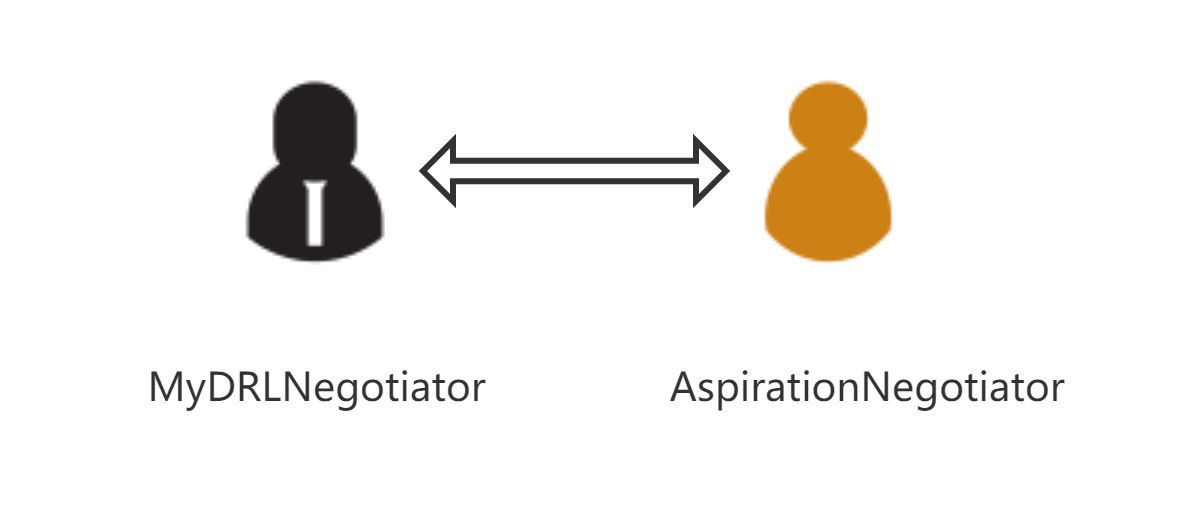
\includegraphics[width=0.50\textwidth]{./images/bilateral-negotiation.png}
\caption{Bilateral Negotiation Game in \gls{sbe}, My Deep Reinforcement Learning Negotiator vs. Aspiration Negotiator}
\label{fig:bilateral-negotiation}
\end{figure}

Negotiation mechanism is \gls{saom}, RL negotiator can learn two strategies called \textbf{acceptance strategy} and \textbf{offer strategy}, which will be described in detail in the following paragraphs. 

\paragraph{Acceptance strategy} actions of agent are \texttt{Accept offer}, \texttt{Wait} and \texttt{Reject offer}. The variables observed by the agent are current offer of opponent and current time(running time, or relative round of negotiation mechanism).

\paragraph{Offer strategy} Actions of negotiator are set of outcome in negotiation mechanism. The observation is same as observation defined in the acceptance strategy. Before feeding variables into the algorithm, action and observation are normalized.

\subsubsection{single issue}
The training environment is based on the \gls{sbe} and sets concrete limits and attributes for it, which are defined in table \ref{tab:attributes-sbe}.

\begin{table}[htbp]
\centering
\begin{tabular}{l l l} \toprule
\bfseries \textbf{Attributes}      & \bfseries \textbf{Value}             \\ \midrule
\textbf{Name}                    & negotiation\_env\_ac\_s, negotiation\_env\_of\_s \\
\textbf{Negotiation Mechanism}   & SAOMechanism                                        \\
\textbf{Max\_Steps}              & 100                                                 \\
\textbf{Issue}             	     & Price(300, 550)                                     \\
\textbf{Competitors}             & [MyDRLNegotiator, AspirationNegotiator]             \\
\textbf{Utility Functions}       & [LinearUtility(-0.35), LinearUtility(0.25)]         \\
\textbf{Actions}                 & [ACCEPT, REJCT, WAIT, END], Outcomes\\
\bottomrule
\end{tabular}
\caption{Attributes of the training environment(sbe), single-issue}
\label{tab:attributes-sbe}
\end{table}

Algorithms \gls{dqn}, \gls{ppo}, ACER\parencite{DBLP:journals/corr/WangBHMMKF16}, A2C and DDPG are tested in the cases of single issue. The curve of mean episode reward of case  \textbf{single issue, acceptance strategy} and \textbf{single issue, offer strategy} are shown in \ref{fig:single-issue}. \gls{dqn}, ACER, \gls{ppo} and A2C support the discrete action space. Hence, these algorithms are used for training acceptance strategy, its action space is discrete. Additionally, \gls{ddpg}, \gls{ppo} and A2C can be used for training offer strategy, its action spaces can be considered as continuous. The curve of mean epsidoe reward is represented as two type: 
\begin{itemize}
\item step: combine mean episode reward of all algorithms into one figure
\item wall: split the mean episode reward of all algorithms as horizontal independente figure.
\end{itemize}

\begin{figure}
    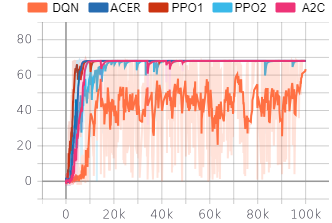
\includegraphics[width=.44\textwidth]{./images/ac_s.png}\hfill
    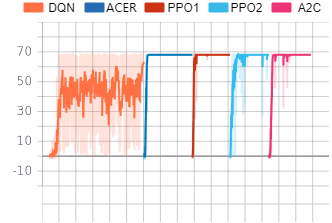
\includegraphics[width=.44\textwidth]{./images/ac_s_wall.png}
    \\[\smallskipamount]
    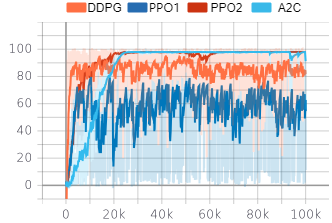
\includegraphics[width=.44\textwidth]{./images/of_s.png}\hfill
    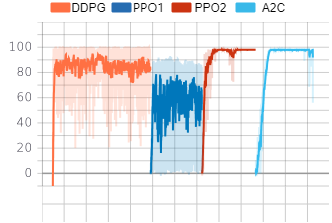
\includegraphics[width=.44\textwidth]{./images/of_s_wall.png}
    \caption{Mean reward of \textbf{Acceptance Strategy}(top left(step), top right(wall)) and of \textbf{Offer Strategy}(bottom left(step), bottom right(wall)) under single issue negotiation}
		\label{fig:single-issue}
\end{figure}

\paragraph{Evaluation} When training independent negotiator with SAOMechanism in the environment \gls{sbe}, almost all well-known \gls{drl} algorithms have the ability to learn. \gls{acer}, \gls{ppo} and A2C have learned very good acceptance strategy, the mean reward curve converged to around 70(i.e., 68.9). However, the performance of dqn is not particularly good. For learning offer strategy, PPO2(improved version of \gls{ppo}) and A2C perform best. The reward curve converged to around 100. The result of \gls{ddpg} are also valuable. Although the reward curve does not converge, it oscillates around a better strategy. Overall, normal version \gls{ppo} does not perform well here. 

\subsubsection{multi issues}
The training environment is almost same as the training environment for single issue. It is based on the \gls{sbe} and sets concrete limits and attributes for it, which are defined in table \ref{tab:attributes-sbe-multi-issues}.

\begin{table}[htbp]
\centering
\begin{tabular}{l l l} \toprule
\bfseries \textbf{Attributes}      & \bfseries \textbf{Value}             \\ \midrule
\textbf{Name}                    & negotiation\_env\_ac\_s, negotiation\_env\_of\_s                     \\
\textbf{Negotiation Mechanism}   & SAOMechanism                                                         \\
\textbf{Max\_Steps}              & 100                                                                  \\
\textbf{Issue}             	     & [Quantity(0, 100), Time(0, 100), Price(10, 100)]                     \\
\textbf{Competitors}             & [MyDRLNegotiator, AspirationNegotiator]                              \\
\textbf{Utility Functions}       & [LinearUtility((0, -0.25, -0.6)), LinearUtility((0, 0.25, 1))]       \\
\textbf{Actions}                 & [ACCEPT, REJCT, WAIT, END], Outcomes                                 \\
\bottomrule
\end{tabular}
\caption{Attributes of the training environment(sbe), multi-issues}
\label{tab:attributes-sbe-multi-issues}
\end{table}

As same as under single issue cases, the curve of mean episode reward of case  \textbf{multi-issues, acceptance strategy} and \textbf{multi -issues, offer strategy} are shown in \ref{fig:multi-issues}. 
\begin{figure}
    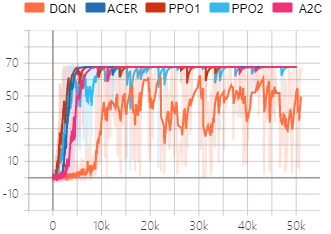
\includegraphics[width=.40\textwidth]{./images/ac_s_multi_issues.png}\hfill
    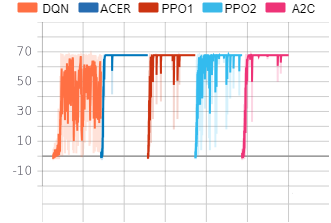
\includegraphics[width=.40\textwidth]{./images/ac_s_multi_issues_wall.png}
    \\[\smallskipamount]
    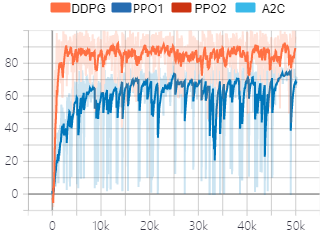
\includegraphics[width=.40\textwidth]{./images/of_s_multi_issues.png}\hfill
    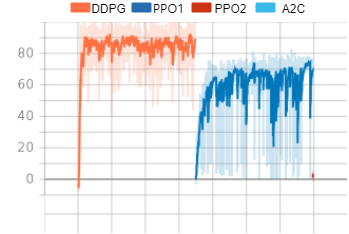
\includegraphics[width=.40\textwidth]{./images/of_s_multi_issues_wall.png}
    \caption{Mean reward of \textbf{Acceptance Strategy}(top left(step), top right(wall)) and of \textbf{Offer Strategy}(bottom left(step), bottom right(wall)) under multi-issues negotiation}
		\label{fig:multi-issues}
\end{figure}

\paragraph{Evaluation} The characteristics of the mean episode reward curve are the same as in single-issue cases. After increasing the action space, the training time increased rapidly. 

\section{Multi-Agent Concurrent Bilateral Negotiation Environment (\gls{mcbe})}
In this environment, agent represents the factory manager and negotiation controller in standard \gls{scml} and \gls{scml} OneShot, respectively.

The agent interacting with environment may be have many related trainable agents(e.g. one seller, one buyer, named as trainer) as the part of learner in the model. Each seller and buyer controls multiple negotiation sessions. The detail of interactive logic is shown below in \ref{fig:interacting-logic-scml}

\begin{figure}[htbp]
\centering
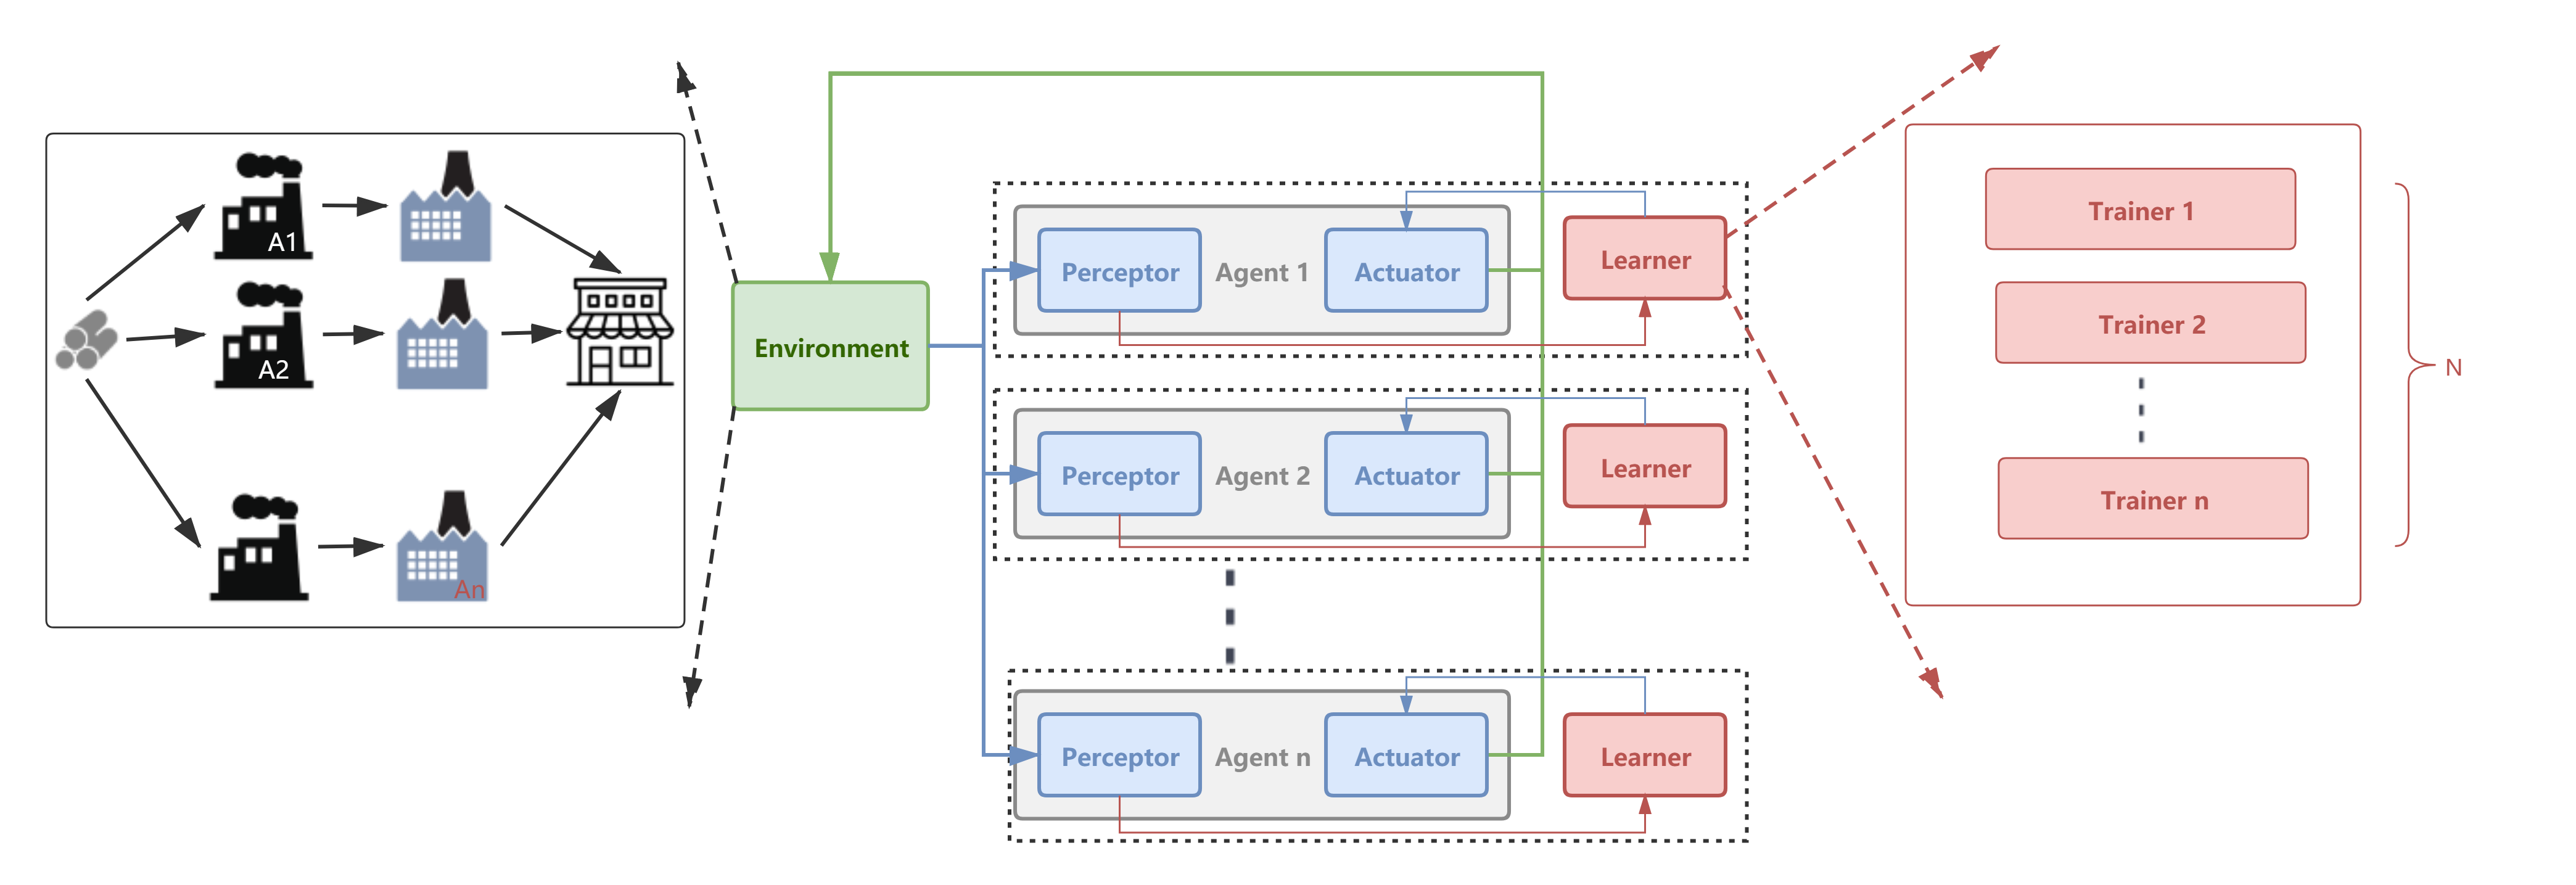
\includegraphics[width=1.0\textwidth]{./images/scnk.png}
\caption{Interactive logic based on the perspective of \gls{scml}. N: The maximum number of concurrent negotiations for a single agent}
\label{fig:interacting-logic-scml}
\end{figure}

Where environment contains six factories and two system entities(SELLER and BUYER). Three RL agents(A1, A2, An) are located at two production positions. Each RL agent contains three parts:

\begin{itemize}
\item \textbf{Perceptor} Receives state, reward from environment and send these to Learner.
\item \textbf{Actuator} Receives action from Learner and execute it in the environment.
\item \textbf{Learner} In addition to connecting with \textbf{Perceptor} and \textbf{Actuator}, it manages the multiple trainer.
\end{itemize}

Based on different algorithms, the internal components of the trainer are different. In general, the trainer will handle the training and execution logic of concurrent negotiation. It will be introduced in the specific algorithm, diagramed in figures \ref{fig:method-maddpg-scml} and \ref{fig:method-qmix-scml}.

\subsection{\gls{maddpg} in \gls{scml}} \label{methods:maddpg}
In the standard scml environment, two questions are tried to be fixed with maddpg. 

\paragraph{Question 1: Dynamical Range Of Negotiation Issues}At the beginning of every negotiation in simulator, agent will determine the range which constraints value interval for negotiation issues. In the experiment, the negotiation issues are \textbf{QUANTITY}, \textbf{PRICE} and \textbf{TIME}. After creating the simulation world, simulator determines the minimum and maximum values for each negotiation issue taken by the entire simulation episode, such as value of \textbf{QUANTITY} between (1, 10), \textbf{PRICE} between (0, 100) and \textbf{TIME} between (0, 100). However, for every negotiation mechanism created inside the entire simulation episode, it has its dynamic range of negotiation issues which affect the negotiation process. This question was raised based on such a situation.

\paragraph{Question 2: The Offer For Every Round}From the description of question 1, we can find, action obtained by algorithm influence only finite the state of environment. Agent(Factory Manager) can not control the function \textbf{proposal} of every negotiation round. Every negotiation round has always been controlled by heuristic negotiation strategy. Intuitively, the main influence comes from the joint action of each round of the negotiation. Hence, question 2 \textbf{The Offer For Every Round} is proposed naturally. After the basic problem is determined, how to design becomes the current problem. 

From an algorithm perspective, the data flow of the model is shown in \ref{fig:method-maddpg-scml}. 
\gls{maddpg} used in \gls{scml}, one trainable agent(trainer) defined in \gls{maddpg} is not equal to the agent defined in \gls{scml}.
It create $D$ process for action exploration, in this environment, \textbf{Dynamical Range Of Negotiation Issues}(Question 1) and \textbf{The Offer For Every Round}(Question 2) are needed to be explored.
The basic concepts of \gls{maddpg} are introduced in chapter background \ref{background:maddpg}. 

\begin{figure}[htbp]
\centering
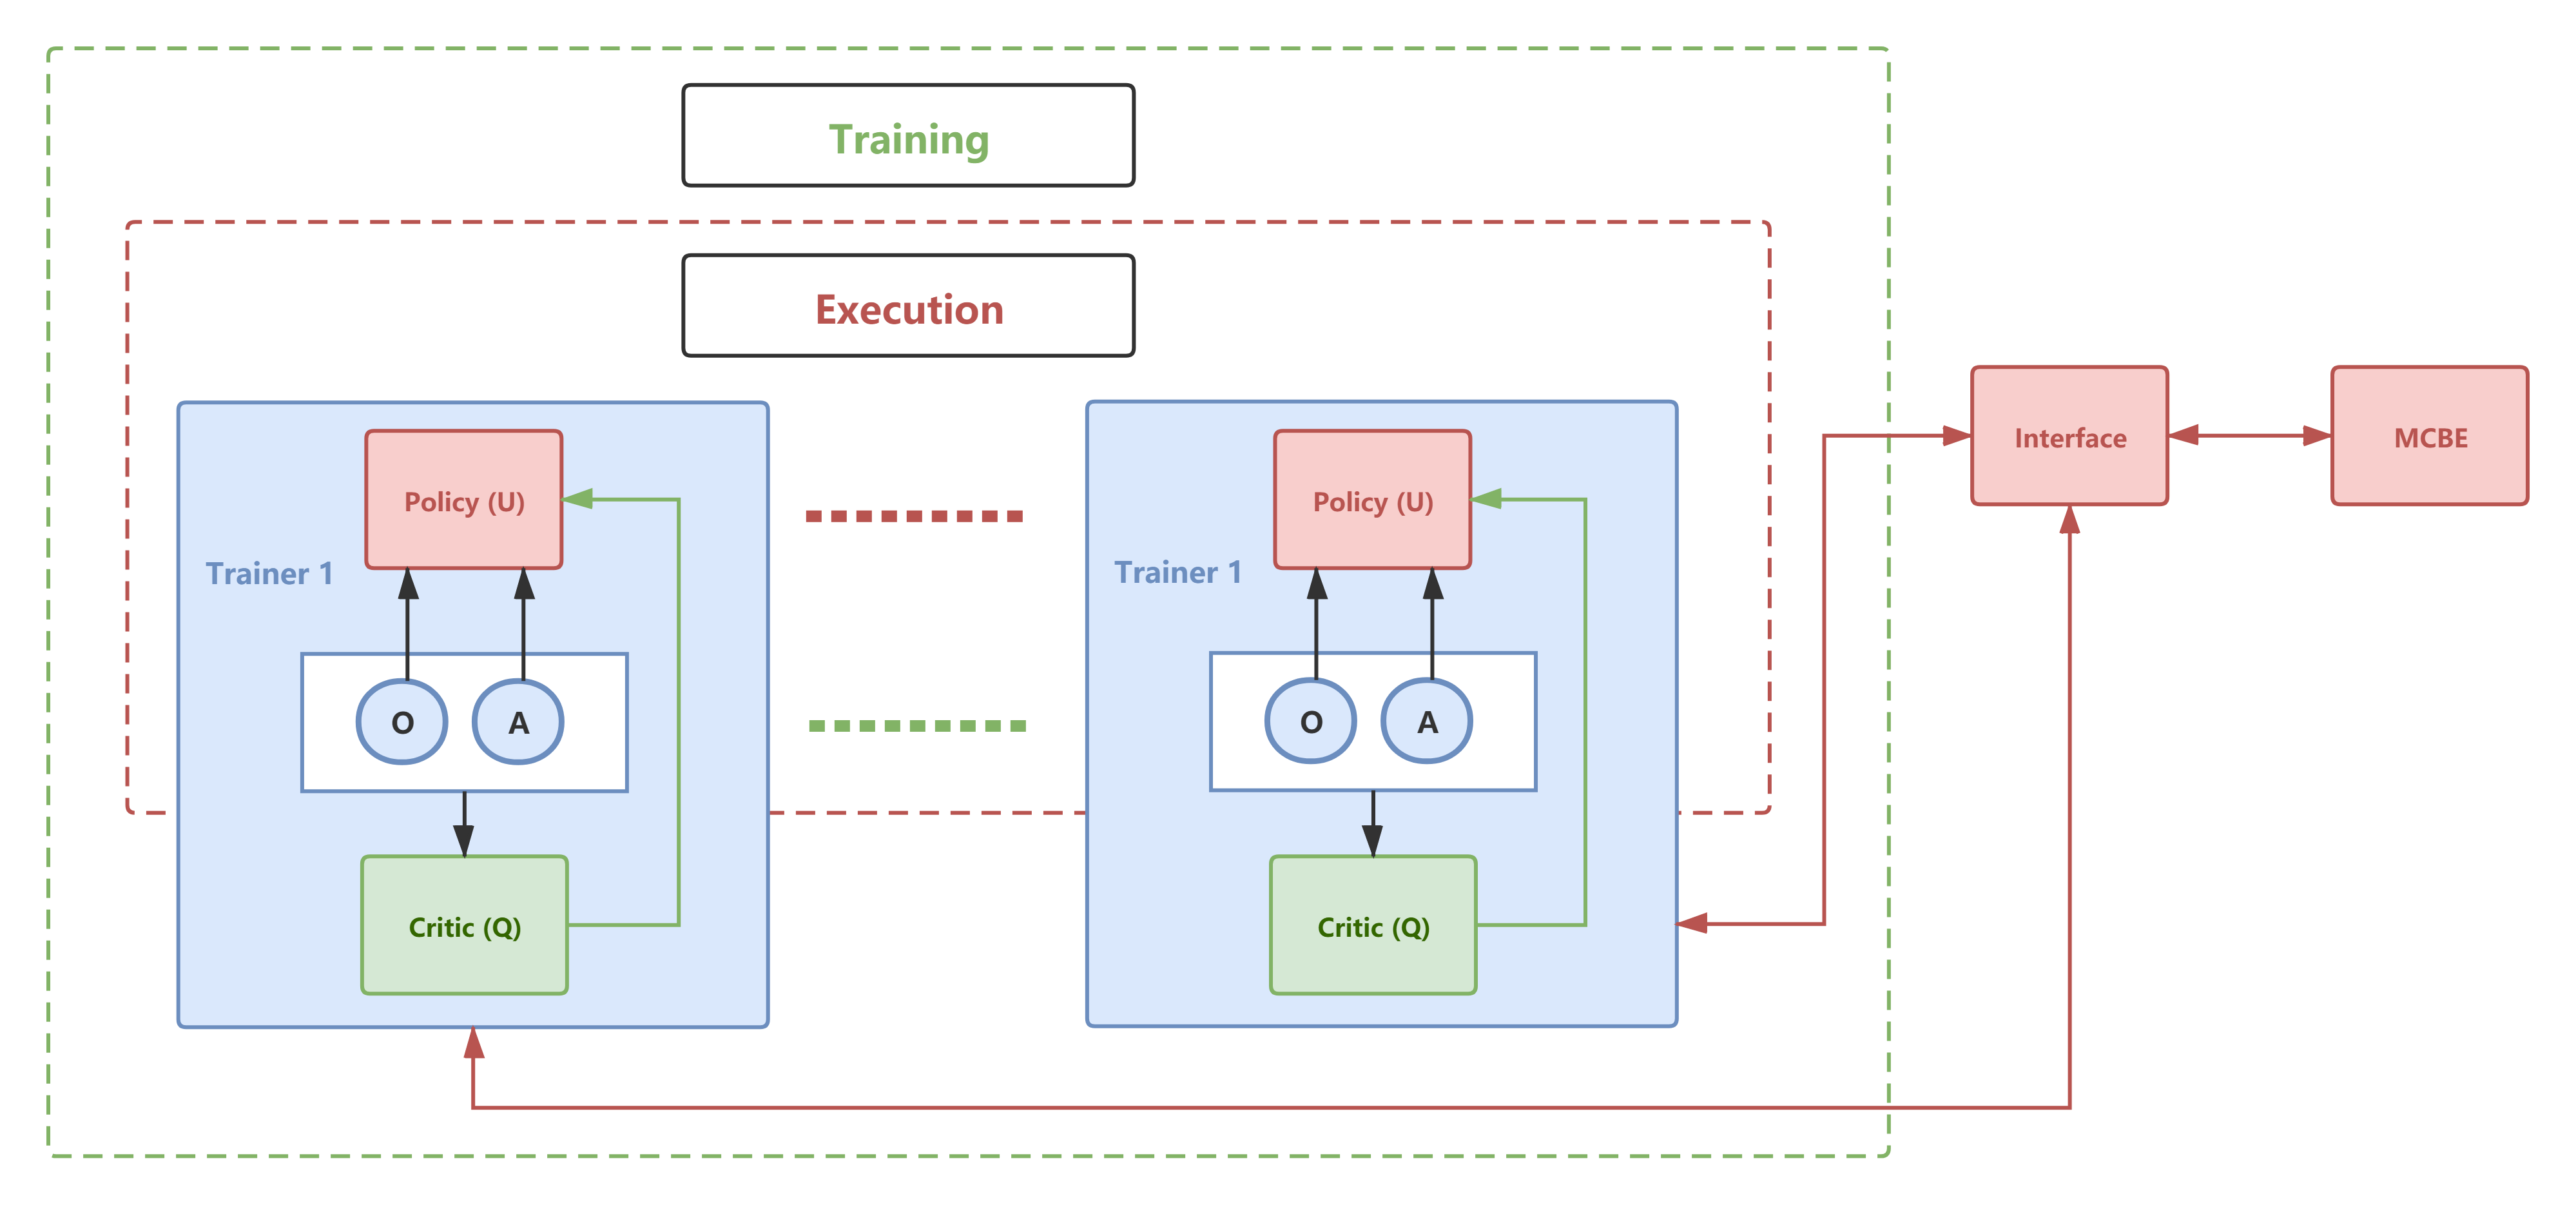
\includegraphics[width=1.00\textwidth]{./images/scml-maddpg.png}
\caption{\gls{maddpg} used in \gls{mcbe}}
\label{fig:method-maddpg-scml}
\end{figure}

In the model \ref{fig:method-maddpg-scml}, policy output action as input to related agent interacting with the environment, which outputs the observation and reward as the inputs to related trainer. Two trainers are created in the experiment:
\begin{itemize}
\item \textbf{trainer\_seller} controls all sale negotiations, the size of the action space has a linear relationship with the size of the largest concurrent sale negotiations.
\item \textbf{trainer\_buyer} controls all buy negotiations, the size of the action space has a linear relationship with the size of the largest concurrent purchase negotiations.
\end{itemize}

Details of the algorithm are described in the appendix \ref{appendix:algorithms:maddpg}.  


\subsection{\gls{qmix} in \gls{scml-oneshot}} \label{methods:qmix-scml-oneshot}

The world created by \gls{scml-oneshot} is described in detail in chapter background \ref{background-scml}. 

\paragraph{Question: The Offer For Every Step} Unlike in standard scml \textbf{Dynamical Range of Negotiation Issues} is controlled by agents, the system takes over the related control and access authority in scml oneshot. Hence, question 1 in the standard library does not need to be discussed here. Although the design of oneshot world is very different with the standard libray, the key question is also how to find the optimal sequence action(offer for every negotiation step).

In the current version \gls{qmix}, which is used in the experiment, one trainable agent is related to one negotiation session. When the agents are located in different locations in the scml world, the agents have different concurrent negotiation maximums. Since the agent \textbf{A1} shown in Figure \ref{fig:interacting-logic-scml} has three consumers, the maximum value of concurrent negotiations of the agent \textbf{A1} is 3. Based on this value, we need to create three trainable agents in algorithm, and each trainable agent control one negotiation session of interative agent.

Data flow is shown in \ref{fig:method-qmix-scml}, the total number of trainers is equal to the sum of the most simultaneous negotiations of all agents. Additionally, unlike in maddpg, in qmix, there is only one global learner, which can control all trainers together.

\begin{figure}[htbp]
\centering
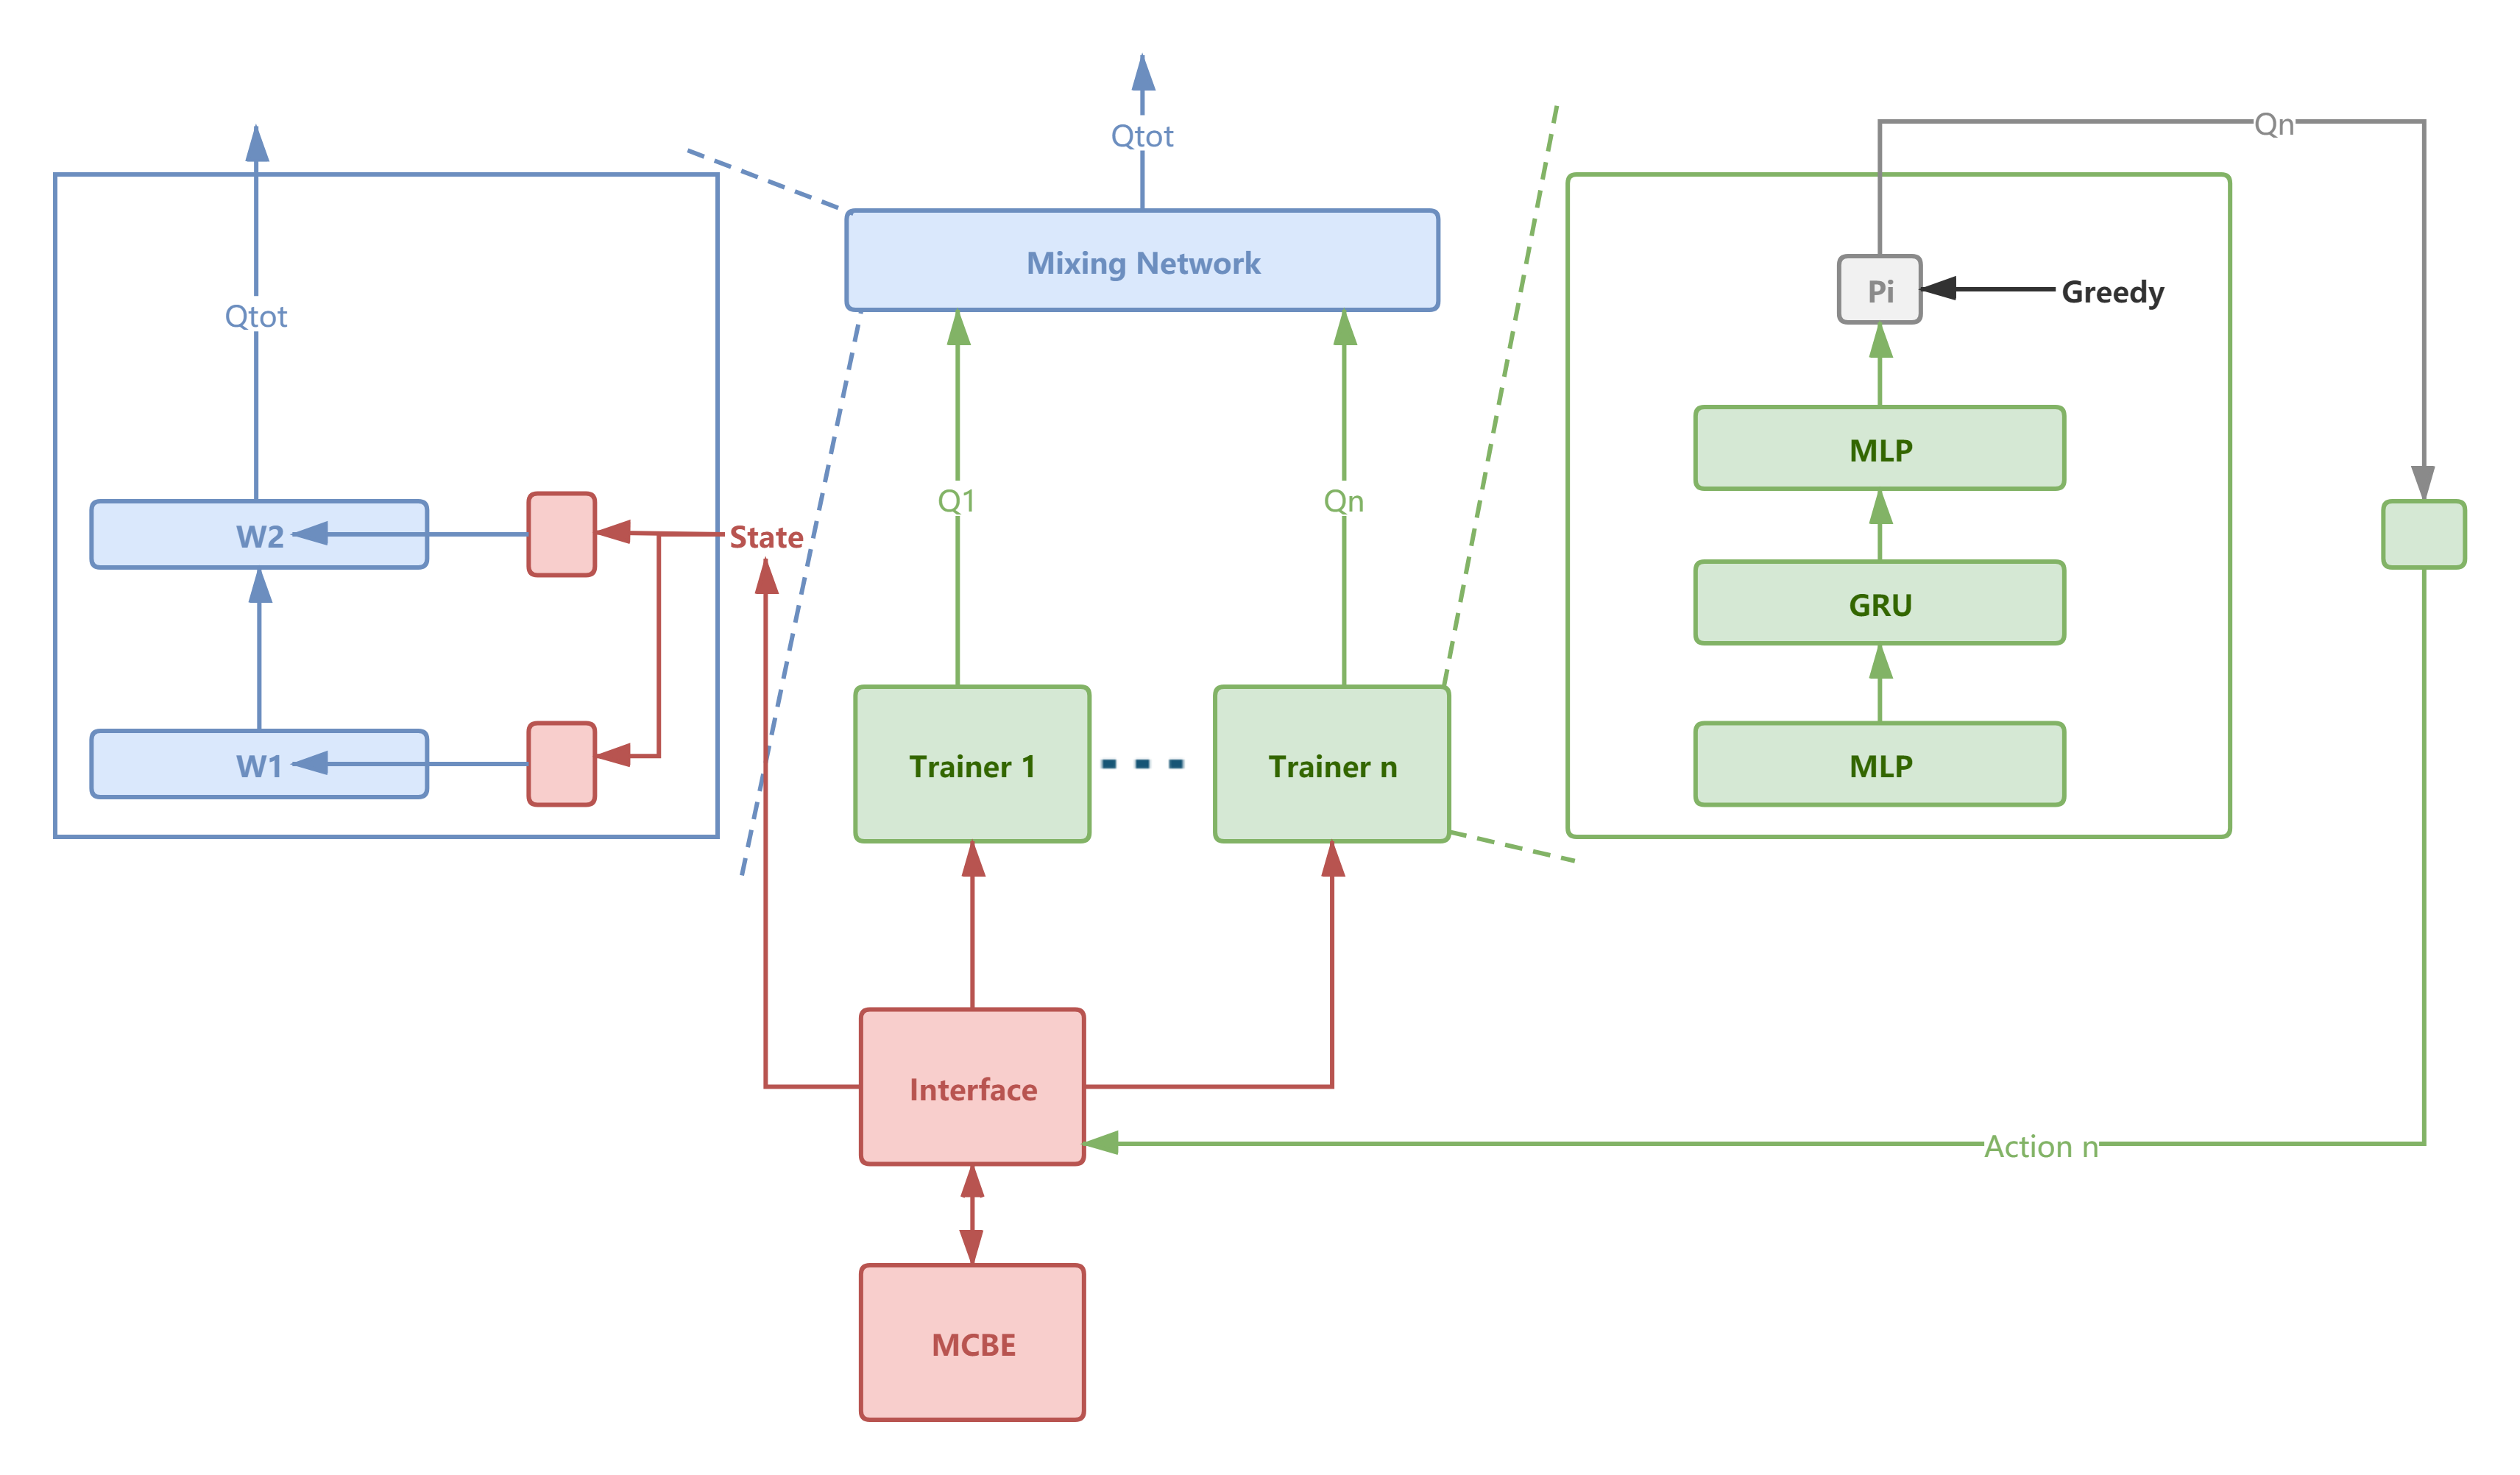
\includegraphics[width=0.80\textwidth]{./images/scml-qmix.png}
\caption{\gls{qmix} used in \gls{mcbe}}
\label{fig:method-qmix-scml}
\end{figure}

\subsection{Experiment}
\subsubsection{Concurrent Neogtiations in standard \gls{scml}}
Standard \gls{scml} is a complex simulation world, which contains various parts with specific functions. The breif description of this simulation is introduced in chapter Background \ref{background-scml}. The experiment of this thesis focus on only the Negotiation Manager(Negotiation Control Strategy) of Decision-Maker Agent. The above mentioned method maddpg \ref{methods:maddpg} is used in this experiment. 
Scenario is diagramed in Figure \ref{fig:scenario-standard-scml}.

\begin{figure}[htbp]
\centering
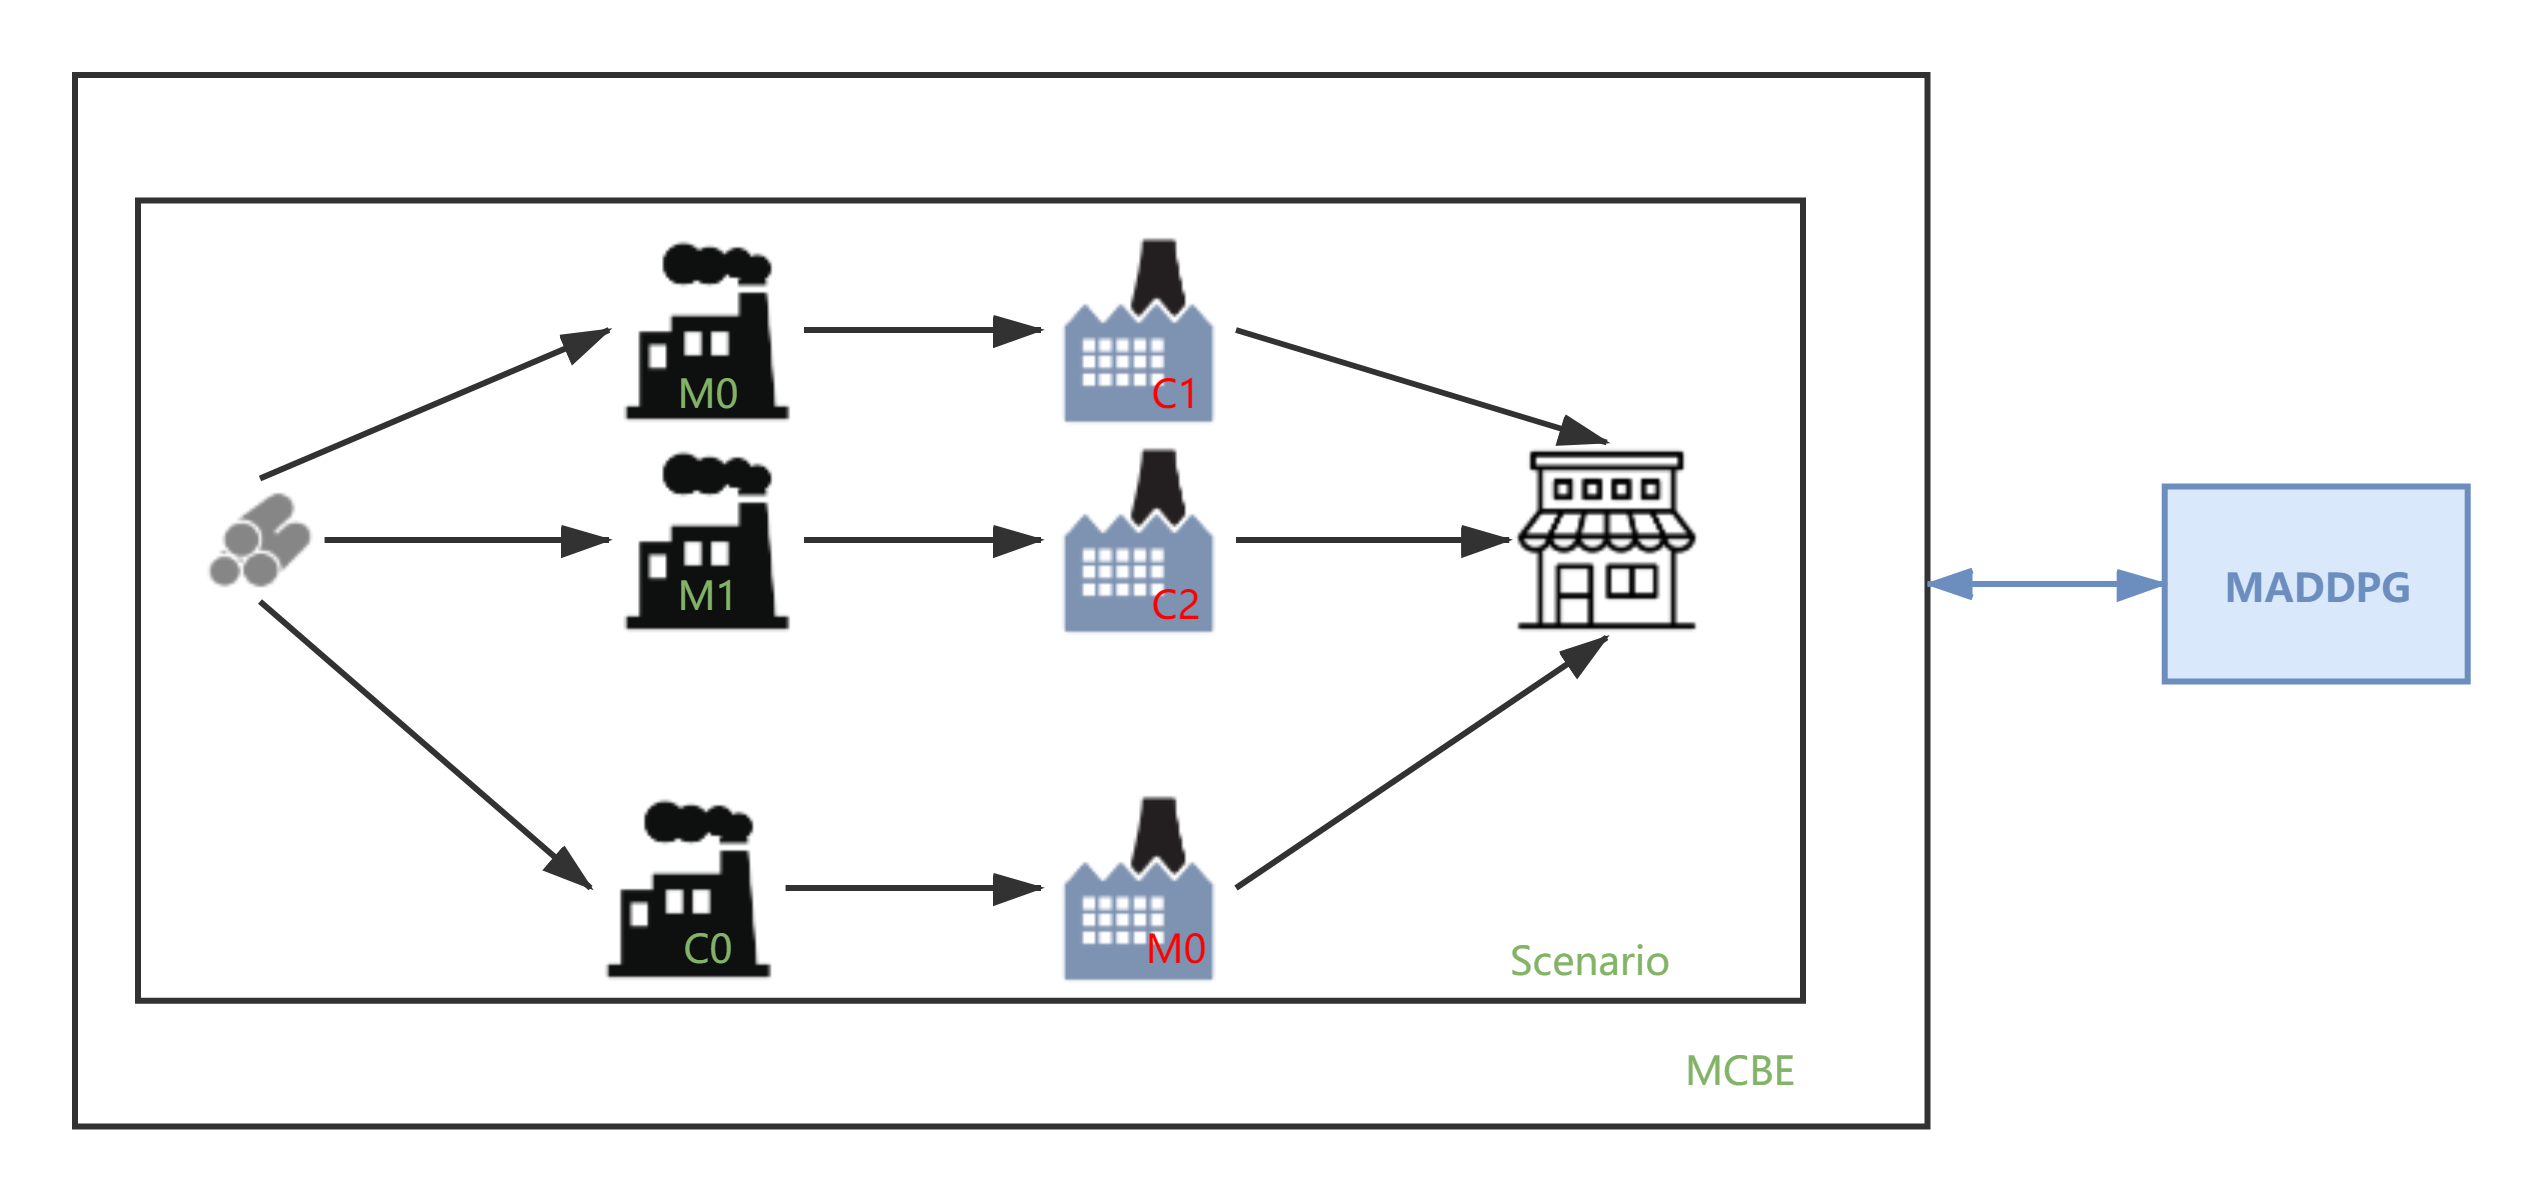
\includegraphics[width=0.80\textwidth]{./images/scenario-standard-scml.png}
\caption{M* represent My Component Based Agent with learner \gls{maddpg}, C* represent Opponent Agents, such as \gls{ind-dec-agent}}
\label{fig:scenario-standard-scml}
\end{figure}

The training environment is based on the \gls{mcbe} and sets concrete limits and attributes for it, which are defined in table \ref{tab:attributes-mcbe-dynamical-range-negotiation-issue}.

\begin{table}[htbp]
\centering
\begin{tabular}{l l l} \toprule
\bfseries \textbf{Attributes}    & \bfseries \textbf{Value}                                             \\ \midrule
\textbf{Name}                    & scml                                                                 \\
\textbf{World}                   & SCML2020World                                                        \\
\textbf{Neogitation Mechanism}   & SAOMechanism                                                         \\
\textbf{Max Negotiation Steps}   & 10                                                                   \\
\textbf{Max Simulation Steps}    & 10                                                                   \\
\textbf{Issue}             	     & [Quantity(0, 100), Time(0, 100), Price(10, 100)]                     \\
\textbf{Competitors}             & [MyBasedAgent, DecentralizingAgent]                                  \\
\textbf{Negotiated Rate}         &    1                                                                 \\
\textbf{DNSP}                    &    True                             \\
\textbf{Actions}                 & Range of Negotiation Issues                                          \\
\bottomrule
\end{tabular}
\caption{Attributes of the training environment(mcbe), DNSP: Disallow Negotiation with Same Partners, standard scml}
\label{tab:attributes-mcbe-dynamical-range-negotiation-issue}
\end{table}

\paragraph{Evaluation of Question1:} The result of training of case Question 1 \textbf{Dynamical Range Of Negotiation Issues} proposed in section \ref{methods:maddpg} is shown in \ref{fig:dynamical-range-issues-maddpg}. From the mean episode reward curve we can know that the agent learns nothing in this case. It means, merely changing the dynamic range of negotiation issues cannot effectively improve agent strategy. Compared with baseline agent IndDecentralizingAgent, the score of MyComponentsBasedAgent is not obvious better.  

\paragraph{Evaluation of Question 2:}  
 
Overall, idea from maddpg is very constructive, but it is difficult to learn good strategies using maddpg. Training consumes a lot of time and hardware resources.


\begin{figure}
    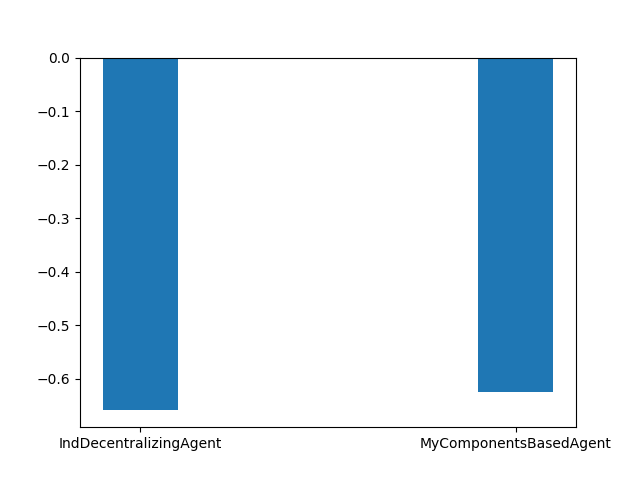
\includegraphics[width=.45\textwidth]{./images/dynamic_range_issues_maddpg.png}\hfill
    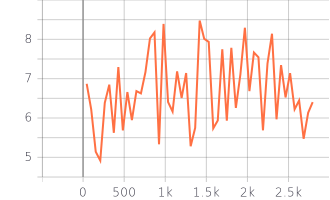
\includegraphics[width=.49\textwidth]{./images/dynamical_mean_episode_reward.png}
    \caption{Scores(left) of agents running in simulation world after training, Mean Episode Reward(right)}
		\label{fig:dynamical-range-issues-maddpg}
\end{figure}

\subsubsection{Concurrent Negotiations in OneShot \gls{scml}}
\gls{scml-oneshot} world is a new simpler world from standard scml. This world only cares about concurrent negotiation in supply chain management, and the agents used in this world can be easily transferred to standard scml. 
 
The breif description of this simulation world is introduced in chapter Background \ref{background-scml}. This part of the experiment only focuses on negotiation. The above mentioned method qmix \ref{methods:qmix-scml-oneshot} is used in this experiment. 

\paragraph{self-play}

Scenario is diagramed in Figure \ref{fig:scenario-oneshot-scml-self-play}.
\begin{figure}[htbp]
\centering
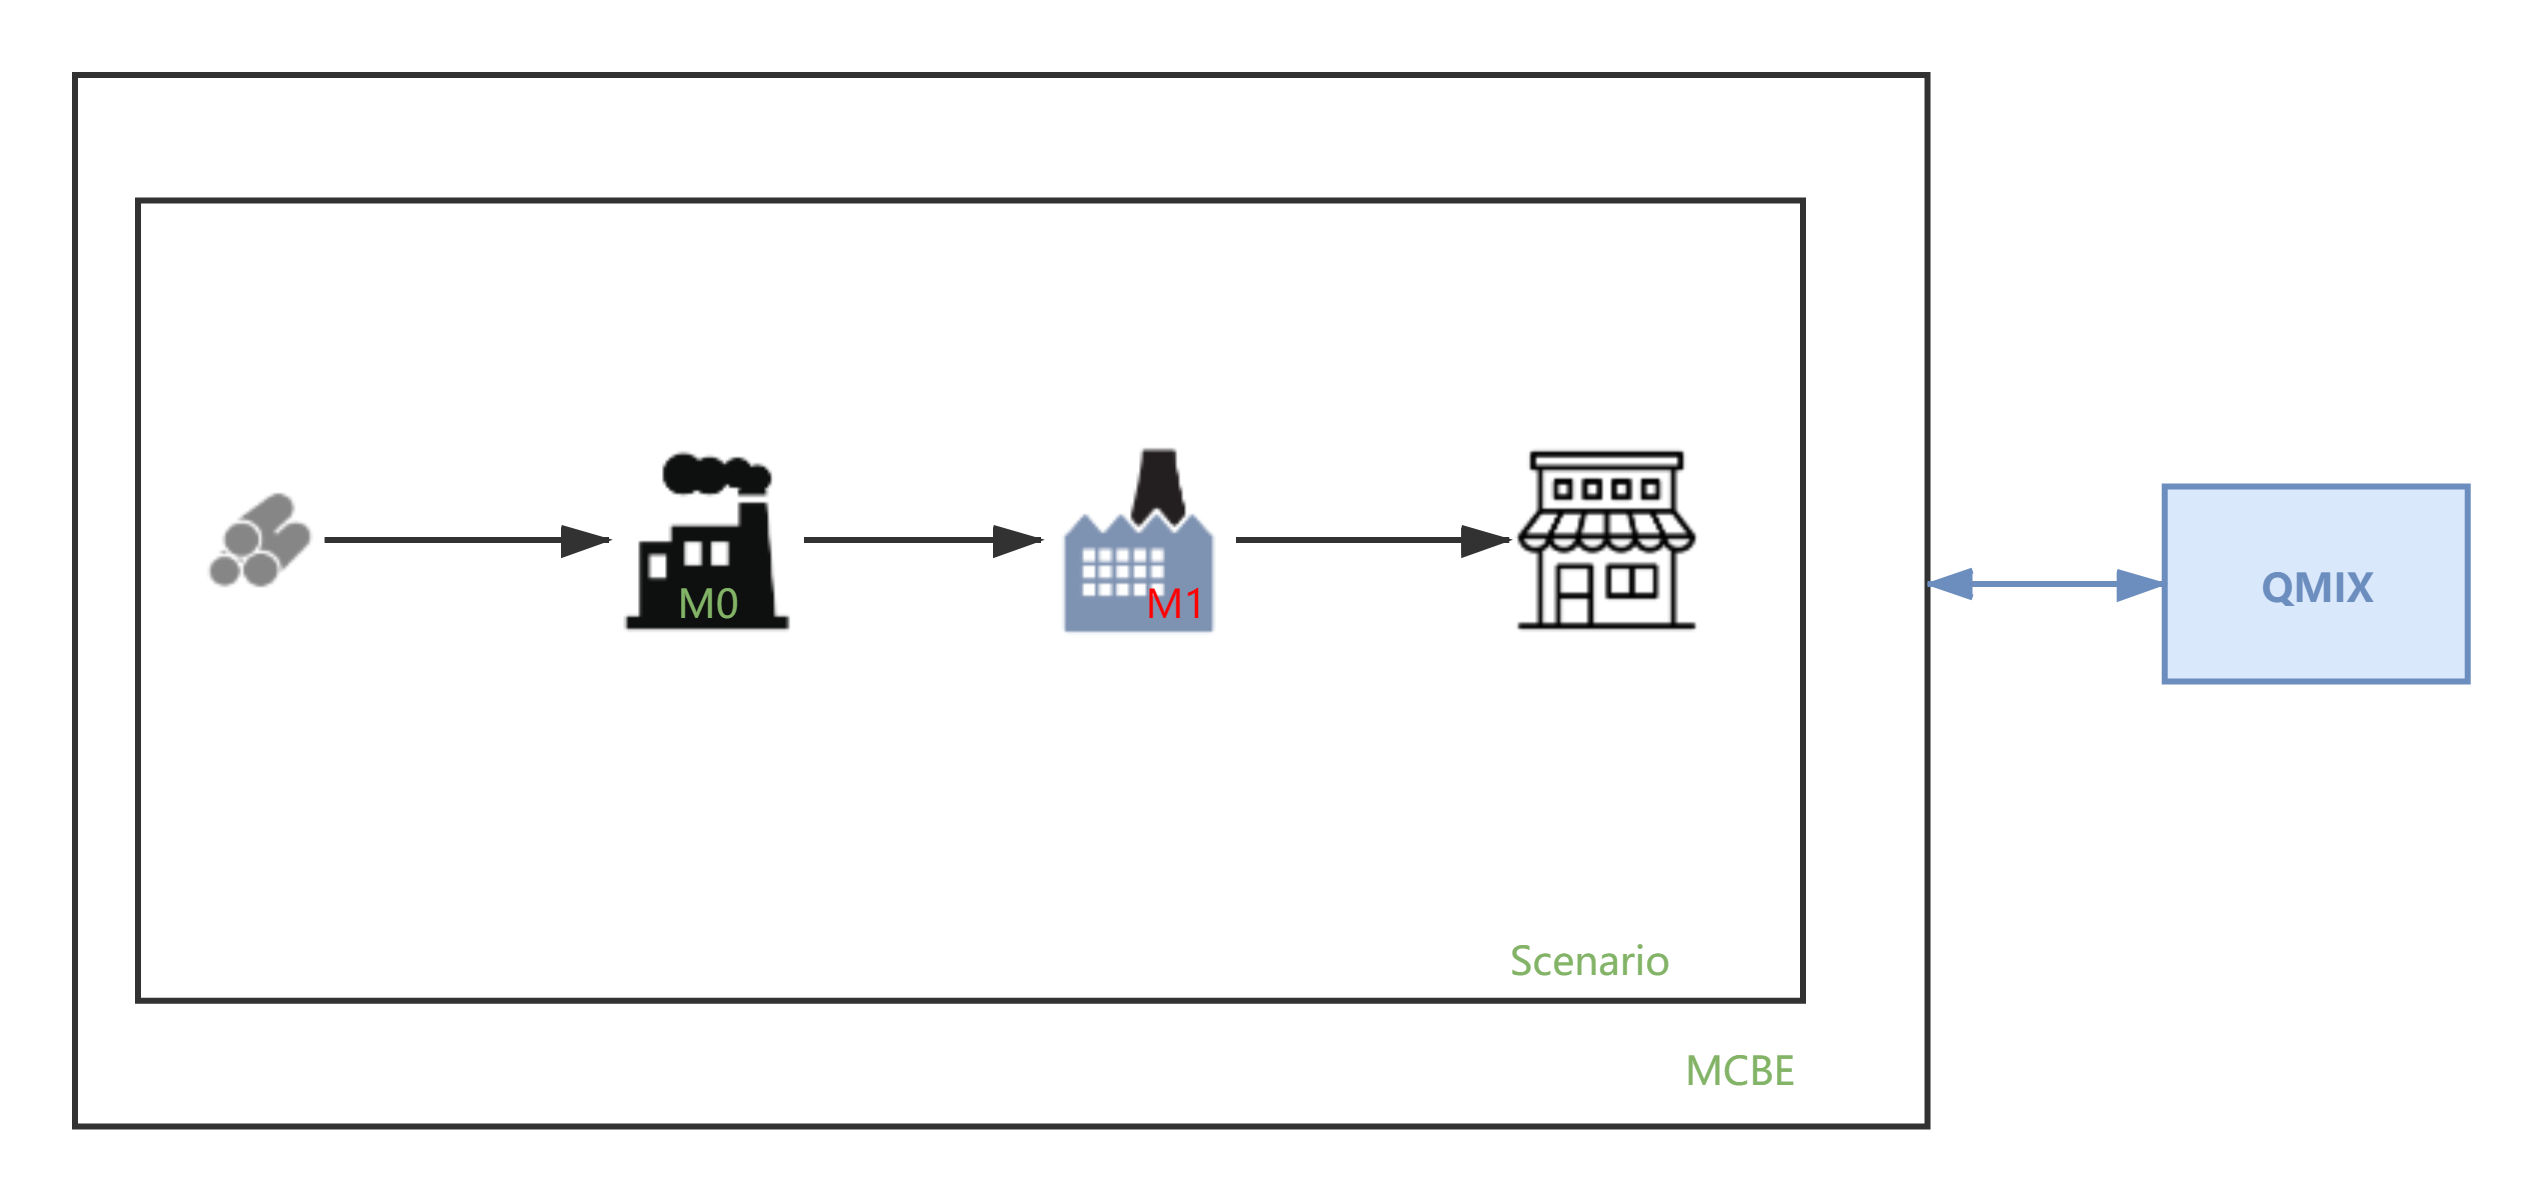
\includegraphics[width=0.80\textwidth]{./images/scenario-oneshot-scml-self-play.png}
\caption{M* represent My Component Based Agent with learner \gls{qmix}}
\label{fig:scenario-oneshot-scml-self-play}
\end{figure}

The training environment is based on the MCBE and sets concrete limits and attributes for it,
which are defined in table \ref{tab:attributes-mcbe-concurrent-negotiation-scml-oneshot}.

\begin{table}[htbp]
\centering
\begin{tabular}{l l l} \toprule
\bfseries \textbf{Attributes}    & \bfseries \textbf{Value}                                             \\ \midrule
\textbf{Name}                    & scml-oneshot-concurrent-negotiation                                  \\
\textbf{World}                   & SCML2020OneShotWorld                                                 \\
\textbf{Neogitation Mechanism}   & SAOMechanism                                                         \\
\textbf{Max Negotiation Steps}   & 20                                                                  \\
\textbf{Max Simulation Steps}    & 100                                                                   \\
\textbf{Issue}             	     & [Quantity(0, 100), Time(0, 100), Price(10, 100)]                     \\
\textbf{Competitors}             & [MyAgent, MyAgent] (self-play)                                       \\
\textbf{Actions}                 & Joint-Outcomes                                                             \\
\bottomrule
\end{tabular}
\caption{Attributes of the training environment(mcbe), scml-oneshot, self-play}
\label{tab:attributes-mcbe-concurrent-negotiation-scml-oneshot}
\end{table}

Episode mean reward curve is shown in \ref{fig:oneshot-self-play}

\begin{figure}[htbp]
\centering
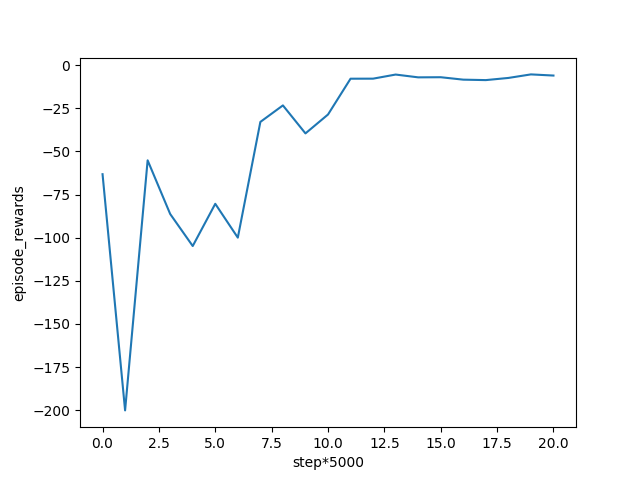
\includegraphics[width=0.55\textwidth]{./images/oneshot_self_play.png}
\caption{Episode mean reward of self paly under SCML OneShot}
\label{fig:oneshot-self-play}
\end{figure}

\paragraph{play with other agent} In this scenario, the opponent agent is a heuristic agent from the scml packages, such as GreedyAgent.
Scenario is diagramed in Figure \ref{fig:scenario-oneshot-scml-play-with-greedy}.
\begin{figure}[htbp]
\centering
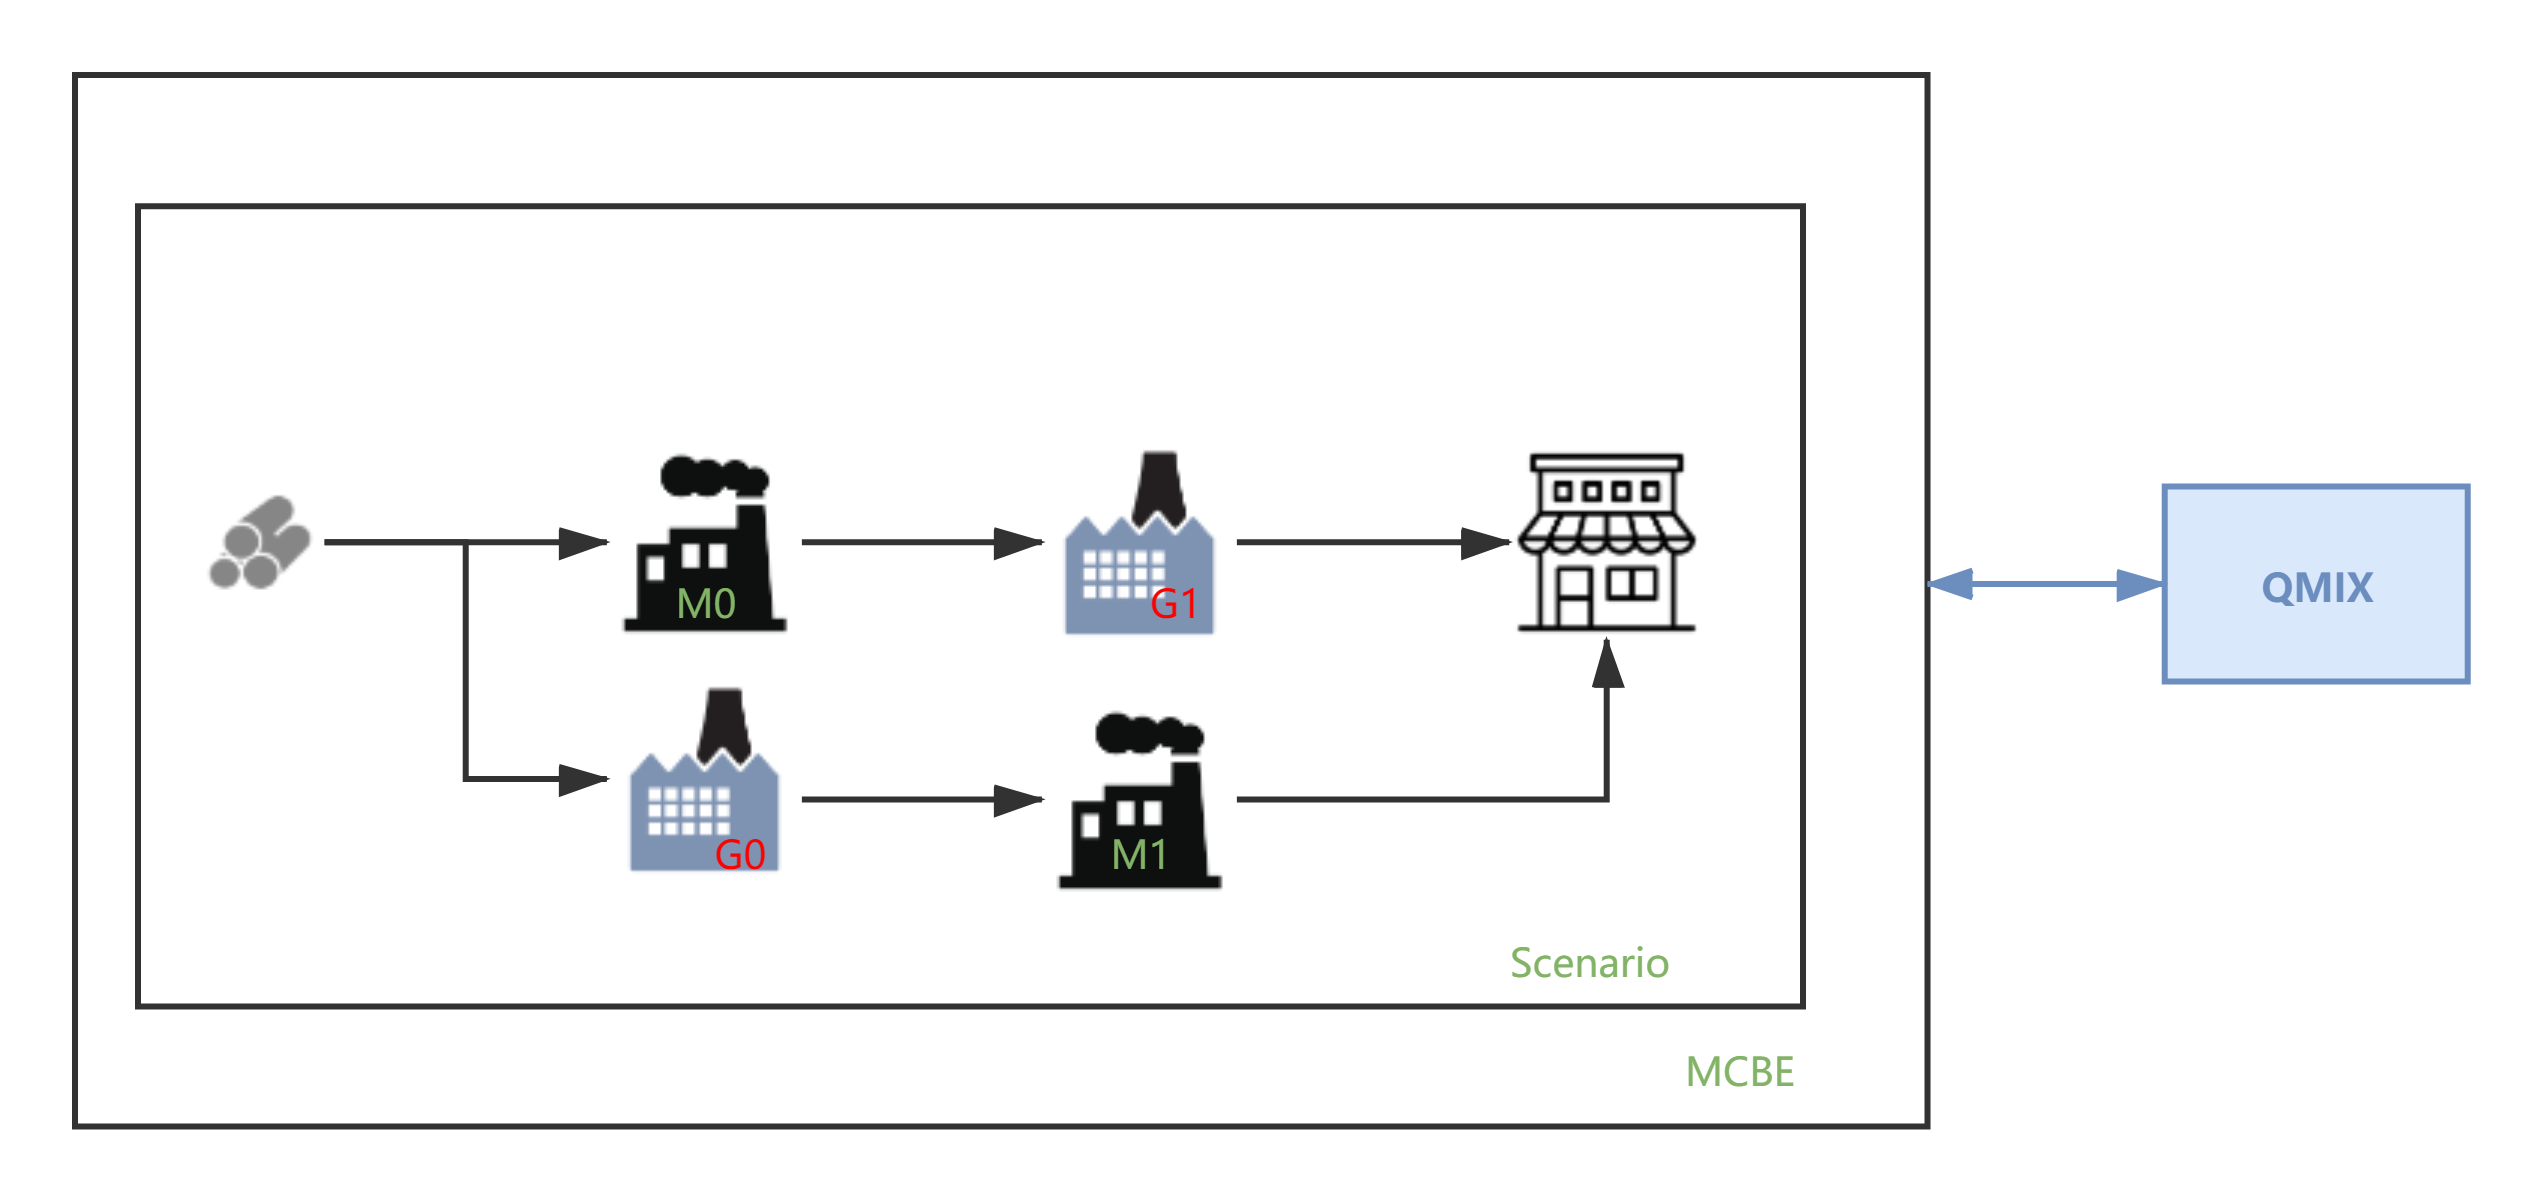
\includegraphics[width=0.80\textwidth]{./images/scenario-oneshot-scml-play-with-greedy.png}
\caption{M* represent My Component Based Agent with learner \gls{qmix}, G* represent GreedyOneShotAgent}
\label{fig:scenario-oneshot-scml-play-with-greedy}
\end{figure}

The training environment is based on the MCBE and sets concrete limits and attributes for it,
which are defined in table \ref{tab:attributes-mcbe-concurrent-negotiation-scml-oneshot-with-others}.

\begin{table}[htbp]
\centering
\begin{tabular}{l l l} \toprule
\bfseries \textbf{Attributes}    & \bfseries \textbf{Value}                                             \\ \midrule
\textbf{Name}                    & scml-oneshot-concurrent-negotiation                                  \\
\textbf{World}                   & SCML2020OneShotWorld                                                 \\
\textbf{Neogitation Mechanism}   & SAOMechanism                                                         \\
\textbf{Max Negotiation Steps}   & 20                                                                  \\
\textbf{Max Simulation Steps}    & 100                                                                   \\
\textbf{Issue}             	     & [Quantity(0, 100), Time(0, 100), Price(10, 100)]                     \\
\textbf{Competitors}             & [MyAgent, GreedyAgent] (play-with-others)                                       \\
\textbf{Actions}                 & Joint-Outcomes                                                             \\
\bottomrule
\end{tabular}
\caption{Attributes of the training environment(mcbe), scml-oneshot, play-with-others}
\label{tab:attributes-mcbe-concurrent-negotiation-scml-oneshot-with-others}
\end{table}

Episode mean reward curve is shown in \ref{fig:oneshot-my-vs-greedy}

\begin{figure}[htbp]
\centering
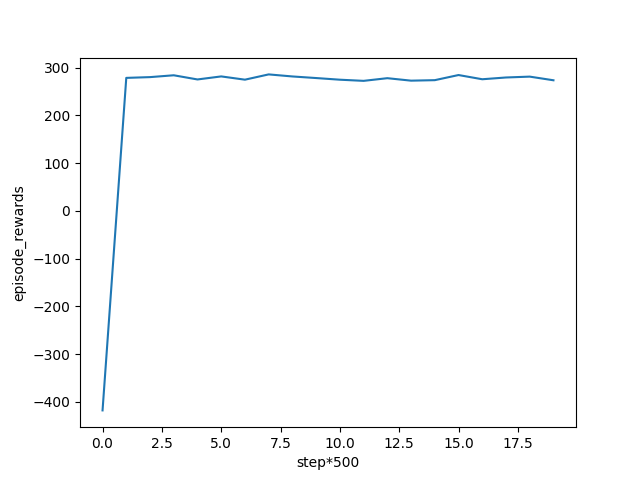
\includegraphics[width=0.65\textwidth]{./images/oneshot_my_vs_greedy.png}
\caption{Episode mean reward of my agent vs GreedyOneShotAgent under SCML OneShot}
\label{fig:oneshot-my-vs-greedy}
\end{figure}

\paragraph{Evaluation} In the scenario \textbf{self-play} and \textbf{play with other agent}, agents learned good strategy. It means method \gls{qmix} is valid in \gls{scm} world.


\section{Conclusion}
The training effect of single agent(negotiator) is not bad. But for multi-agent concurrent negotiations it is not easy to implemente. The work of this thesis focus on just two algortims \gls{maddpg} and \gls{qmix}. The performance and results of \gls{qmix} have certain reference value. In the future many work and algorithms are needed to be finished and implemented in the environment \gls{mcbe}.